%% Math 2.0: Theory and Practice
%% Requires compilation with XeLaTeX or LuaLaTeX:  latexmk main.tex  (see .latexmkrc)
\documentclass[10pt,t,aspectratio=169]{beamer}
\usetheme{Vidal}
% Section Divider Slide Format
% Background from the "2_Divider Slide" layout in PennEngineering-template-2023.pptx
% (slideLayout9, image4.jpg). The title sits exactly on the page's centre; the
% optional label ("Part I") hangs just above it, so every divider's title is in
% the same place whether or not it has a label.
% Usage: \sectionslide{Part I}{Society}, or \sectionslide{}{Closing} for no label.
\def\vidal@sectionlabelgap{0.35cm}  % gap between label and title
\newcommand{\sectionslide}[2]{%
    {%
    \setbeamertemplate{background}{%
        
\includegraphics[width=\paperwidth,height=\paperheight]{PennEngineering-template-2023/ppt/media/image4.jpg}%
    }%
    \setbeamertemplate{footline}{}%
    \begin{frame}[plain]
        \begin{tikzpicture}[remember picture, overlay]
            \node[anchor=center, inner sep=0pt, align=center, text width=0.8\paperwidth]
                (vidal@sectiontitle) at (current page.center)
                {\usebeamerfont{title}\color{white}#2};
            \node[anchor=south, inner sep=0pt, align=center]
                at ([yshift=\vidal@sectionlabelgap]vidal@sectiontitle.north)
                {\usefont{TU}{\sfdefault}{m}{n}\fontsize{14}{16}\selectfont\color{white!80!PennBlue}#1};
        \end{tikzpicture}%
    \end{frame}
    }%
}

\usetikzlibrary{shadows, arrows.meta}
\usepackage{pgfplots}
\pgfplotsset{compat=1.18}
\usepackage{booktabs, tabularx}

% Problem / response tables (Part I). Y = ragged-right X column.
\newcolumntype{Y}{>{\raggedright\arraybackslash}X}
\newcommand{\rowhead}[1]{\leavevmode{\bfseries\color{black}\hyphenpenalty=10000 #1}}
\newcommand{\tabhead}[1]{\leavevmode{\sffamily\bfseries\color{black!55}#1}}
% Status labels: a coloured dot plus a word, so status is never colour alone.
\newcommand{\stopen}{\leavevmode{\color{PennRed}\textbullet}\,open}
\newcommand{\stpartial}{\leavevmode{\color{PennGold}\textbullet}\,partial}
\newcommand{\stdone}{\leavevmode{\color{PennGreen}\textbullet}\,in place}

% Diagram styles (pipeline diagrams and similar).
\tikzset{
  stage/.style={draw=#1!55, fill=#1!7, rounded corners=2pt, line width=0.5pt,
                minimum width=2.2cm, minimum height=0.95cm, align=center, inner sep=2pt},
  stage/.default=black,
  note/.style={font=\sffamily\scriptsize, text=black!55},
  flow/.style={-Stealth, line width=0.6pt, draw=#1!60},
  flow/.default=black,
  colhead/.style={font=\sffamily\scriptsize\bfseries, text=black!45},
  lane/.style={font=\sffamily\scriptsize\bfseries, align=right, anchor=east, text=#1},
  span/.style={|-|, line width=0.4pt, draw=black!35},
}

% Collage card: an image on a white mat with a thin border and a soft shadow.
% \collagecard[<tikz options>]{<width>}{<image>} inside a tikzpicture node.
\tikzset{collagecard/.style={inner sep=1.2pt, fill=white, draw=black!18, line width=0.3pt,
    drop shadow={shadow xshift=0.6pt, shadow yshift=-0.8pt, opacity=0.25}}}

% Event timeline (AcadMathSci timeline slides). Colours are sampled from the
% report's Figure 1 so the categories keep their original scheme.
\definecolor{tlBlue}{RGB}{29,84,158}     % AI results
\definecolor{tlGreen}{RGB}{41,114,70}    % community responses
\definecolor{tlOrange}{RGB}{186,75,26}   % publishing and verification
\definecolor{tlPurple}{RGB}{112,55,150}  % access and funding
\definecolor{tlBand}{RGB}{240,242,245}   % alternating month bands
\definecolor{tlAxis}{RGB}{143,153,163}   % axis
\newcommand{\tltitlefont}{\sffamily\bfseries\fontsize{6}{7}\selectfont}
\newcommand{\tldescfont}{\sffamily\fontsize{5.3}{6.3}\selectfont}
\tikzset{
  % event box: white card with a coloured top edge, thin border, soft shadow
  tlbox/.style={draw=#1!40, fill=white, line width=0.4pt, rounded corners=1.2pt,
                inner xsep=2.2pt, inner ysep=2.4pt, align=left,
                drop shadow={shadow xshift=0.5pt, shadow yshift=-0.7pt, opacity=0.3},
                path picture={\fill[#1] (path picture bounding box.north west)
                              rectangle ([yshift=-1.2pt]path picture bounding box.north east);}},
  tldot/.style={circle, fill=#1, draw=white, line width=0.6pt, inner sep=0pt, minimum size=4.6pt},
  tlleader/.style={draw=#1!65, line width=0.5pt},
}
% \tlevent{dot x}{leader end x}{box centre x}{box bottom y}{colour}{text width}{title}{description}
% Draws the leader from the dot on the axis (y=0) to the box's bottom edge, the
% box, and the dot.
\newcommand{\tlevent}[8]{%
  \draw[tlleader=#5] (#1,0) -- (#2,#4);
  \node[tlbox=#5, text width=#6, anchor=south] at (#3,#4)
    {{\tltitlefont\color{#5}#7\par}\vspace{0.6pt}{\tldescfont\color{black!75}#8\par}};
  \node[tldot=#5] at (#1,0) {};
}
% Layer cards (three layers of checking): \node[layer=<colour>] ...; label \node[lbl=<colour>].
\tikzset{
  layer/.style={draw=#1!55, fill=#1!6, line width=0.6pt, rounded corners=2pt,
                minimum height=1.45cm, text width=9.2cm, inner sep=0.25cm, align=left,
                font=\sffamily\footnotesize},
  lbl/.style={font=\sffamily\small\bfseries, text=#1, anchor=east, align=right},
}
% Legend dot for inline use.
\newcommand{\tllegdot}[1]{\tikz[baseline=-0.6ex]\node[tldot=#1]{};}

% ---------------------------------------------------------------------------
% Skeleton helpers. \stub{minutes}{purpose} prints a grey planning note on the
% slide; set \stubsfalse to hide every note before giving the talk.
% ---------------------------------------------------------------------------
\newif\ifstubs
\stubstrue
\newcommand{\stub}[2]{%
  \ifstubs{\color{gray}\small\itshape [\,#1 min\,]\quad #2\par}\fi}

% Part names, used by the divider slides and the overview slide.
\newcommand{\partnameone}{Society}
\newcommand{\partnametwo}{The Lab}

\title[Math 2.0]{Math 2.0}
\subtitle{From Society to the Lab}
\author{Kyle Poe}
\institute{Vidal Lab, University of Pennsylvania}
\date{November 11, 2026}

\begin{document}

\titleslide{
  \begin{frame}
    \titlepage
  \end{frame}
}

\contentslide

% Time budget: 45 min content + 15 min discussion.
% The talk is a tree mapped onto beamer's levels:
%   \part = Opening / Part I / Part II / Closing
%   \section, \subsection = the nodes below them
% Beamer numbers the parts 1--4, so Part I is part=2 and Part II is part=3
% in \tableofcontents (see the overview slide in sections/02-opener-math-2).
% Section files hold one frame per planned slide, with titles as working labels.

\part{Opening}                                 %  7 min
% Opening > Navier--Stokes
\section{Navier--Stokes}

% [1 min] Collage of the announcement and its reception.
\begin{frame}{September 8, 2026: Math changes forever}
  \centering
  \begin{tikzpicture}[x=1cm, y=1cm]
    % bounding box = visible extent of the collage, so it centres on the page
    \useasboundingbox (0.48,0) rectangle (14.25,-6.25);
    \def\img{images/announcement_images}
    % the result: blow-up visualization (background made transparent; original in \img)
    \node at (2.9,-3.1) {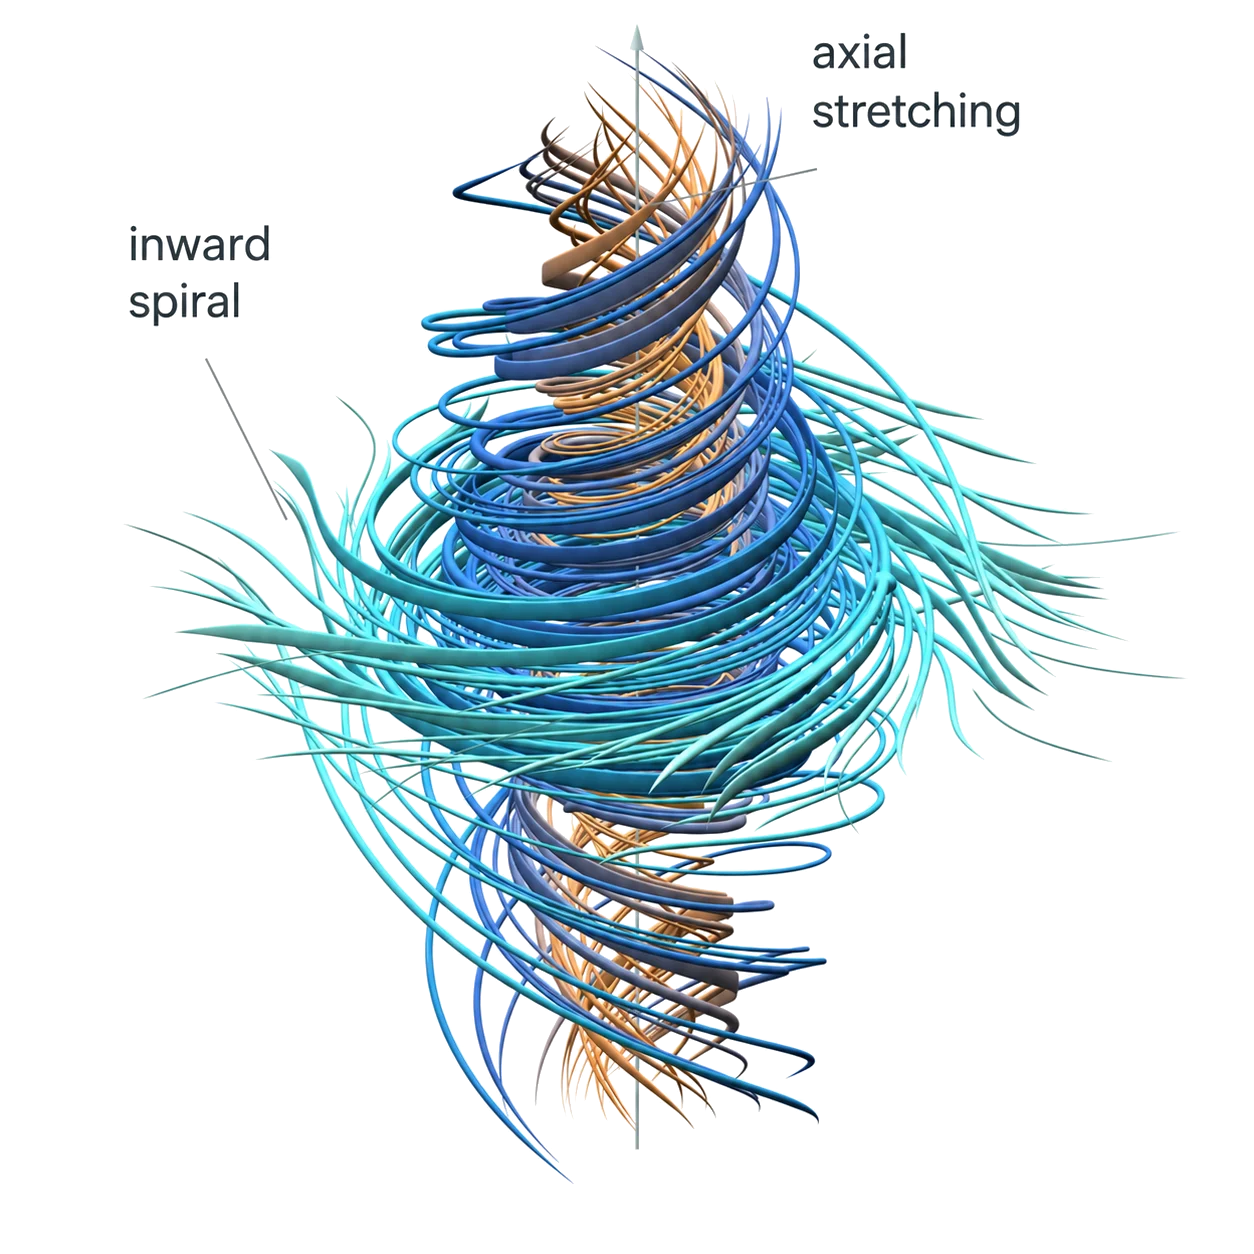
\includegraphics[height=6.1cm]{images/blowup_transparent.png}}; % openai.com/index/navier-stokes-solution/
    % press coverage
    \node[collagecard, rotate=2]    at (8.15,-3.55) {\includegraphics[width=4.9cm]{\img/nature_openai.png}};
    \node[collagecard, rotate=-2.5] at (12.0,-2.95) {\includegraphics[width=4.3cm]{\img/tech_desk_openai.png}};
    \node[collagecard, rotate=1.5]  at (11.2,-5.35) {\includegraphics[width=5.0cm]{\img/forbes_announcement.png}};
    % the announcement itself, on top
    \node[collagecard, rotate=-1]   at (9.6,-0.95)  {\includegraphics[width=7.4cm]{\img/openai_ns_announce.png}};
    % the mood
    \node[collagecard, rotate=-4]   at (6.1,-5.1)   {\includegraphics[width=2.3cm]{\img/cat_discover.png}}; % x.com/MozeTech/status/2097383226503532611
  \end{tikzpicture}
  \slidesources{Sources: OpenAI on X, 8 Sep 2026 \textbullet{} Nature news, 8 Sep 2026 \textbullet{} Technology Desk, 9 Sep 2026 \textbullet{} Forbes \textbullet{} Visualization: OpenAI \textbullet{} Meme: @MozeTech on X}
\end{frame}

% [2 min] The usual route vs OpenAI's route. Builds in three steps:
% (1) the usual route, (2) OpenAI's route skipping peer review, (3) the Lean
% proof sitting in peer review's column, and the takeaway.
\begin{frame}{Why believe it?}
  \centering
  \begin{tikzpicture}[x=1cm, y=1cm, font=\sffamily\footnotesize]
    % bounding box = visible extent of the diagram, so it centres on the page
    \useasboundingbox (0.68,0.1) rectangle (14.01,-6.2);
    % column positions
    \def\ca{2.9}\def\cb{5.4}\def\cc{7.9}\def\cd{10.4}\def\ce{12.9}
    % column headers
    \foreach \x/\t in {\ca/Discovery, \cb/Write-up, \cc/Verification, \cd/Dissemination, \ce/Acceptance}
      \node[colhead] at (\x,-0.15) {\t};

    % ---- (1) the usual route -------------------------------------------------
    \node[lane=black!70] at (1.75,-1.05) {The usual\\route};
    \node[stage] (a1) at (\ca,-1.05) {Human proof};
    \node[stage] (a2) at (\cb,-1.05) {Preprint\\[-1pt]{\scriptsize arXiv}};
    \node[stage] (a3) at (\cc,-1.05) {Peer review\\[-1pt]{\scriptsize referees}};
    \node[stage] (a4) at (\cd,-1.05) {Journal\\[-1pt]{\scriptsize publication}};
    \node[stage] (a5) at (\ce,-1.05) {Accepted\\[-1pt]{\scriptsize Clay: +2 years}};
    \foreach \u/\v in {a1/a2, a2/a3, a3/a4, a4/a5} \draw[flow] (\u) -- (\v);
    \draw[span] (\ca-1.1,-1.85) -- node[note, below=1pt] {months to years} (\ce+1.1,-1.85);

    % ---- (2) OpenAI's route ---------------------------------------------------
    \onslide<2->{
      \node[lane=PennBlue] at (1.75,-3.05) {OpenAI\\Sep 2026};
      \node[stage=PennBlue] (b1) at (\ca,-3.05) {10,000 agents\\[-1pt]{\scriptsize 88 hours}};
      \node[stage=PennBlue] (b2) at (\cb,-3.05) {AI-written\\paper};
      \node[stage, draw=black!35, dashed, fill=white, text=black!40] (b3) at (\cc,-3.05)
        {Peer review\\[-1pt]{\scriptsize skipped}};
      \node[stage=PennBlue] (b4) at (\cd,-3.05) {Announced\\[-1pt]{\scriptsize on X, 8 Sep}};
      \node[stage=PennBlue] (b5) at (\ce,-3.05) {Taken\\seriously};
      \draw[flow=PennBlue] (b1) -- (b2);
      \draw[flow=PennBlue] (b4) -- (b5);
    }
    \only<2>{
      % bypass arc under the skipped box (where the Lean proof appears next)
      \draw[flow=PennBlue] (b2.south east) to[out=-35, in=-145] (b4.south west);
    }

    % ---- (3) what stood in for peer review -----------------------------------
    \onslide<3->{
      \node[stage=PennRed, line width=0.9pt] (b3l) at (\cc,-4.45)
        {\textbf{Lean proof}\\[-1pt]{\scriptsize kernel-checked, +17 h}};
      \draw[flow=PennBlue] (b2.south) |- (b3l.west);
      \draw[flow=PennBlue] (b3l.east) -| (b4.south);
      \draw[span] (\ca-1.1,-5.25) -- node[note, below=1pt] {88 + 17 hours of compute} (\ce+1.1,-5.25);
      \node[font=\sffamily\small, text=PennRed] at (7.1,-6.0)
        {Lean verification, not merely OpenAI's reputation, made the community take this seriously.};
    }
  \end{tikzpicture}
  \slidesources{Sources: OpenAI, 8 Sep 2026 \textbullet{} Reisinger et al., \emph{The Mathematical Sciences in an AI-enabled World}, AcadMathSci, Oct 2026 \textbullet{} Clay Mathematics Institute, Millennium Prize rules}
\end{frame}

       %  3   min
% Opening > An emerging paradigm
\section{An emerging paradigm}

% [1.5 min] Pre-AI history of formal proof as a guarantee. Three rows pair a
% proof that left room for doubt (open circle) with the formal proof that
% settled it (red square); the bar is the lag. Other milestones sit on the
% axis. The AI era is only marked at the right end: slide 5 covers it.
% Every date and quote is from the primary source credited on the right.
\begin{frame}{Timeline: Formalization in the Pre-AI Era}
  \centering
  \begin{tikzpicture}[x=1cm, y=1cm, font=\sffamily\scriptsize,
      doubt/.style={circle, draw=black!55, fill=white, line width=0.6pt, inner sep=0pt, minimum size=4.5pt},
      formal/.style={rectangle, fill=PennRed, inner sep=0pt, minimum size=4.5pt},
      lag/.style={line width=2.4pt, draw=black!12},
      lagtext/.style={font=\sffamily\scriptsize\bfseries, text=black!45, fill=white, inner sep=1pt},
      doubttext/.style={align=left, text=black!65, inner sep=0pt},
      formaltext/.style={align=left, text=PennRed, inner sep=0pt},
      landmark/.style={circle, fill=black!55, inner sep=0pt, minimum size=3pt},
      leader/.style={draw=black!25, line width=0.4pt},
      ltext/.style={text=black!65, inner sep=0pt}]
    % bounding box = visible extent of the diagram, so it centres on the page
    \useasboundingbox (0.87,-0.25) rectangle (14.38,-6.0);

    % ---- row labels and legend (left column) ---------------------------------
    \node[lane=black!70] at (2.85,-0.7) {Four colour\\theorem};
    \node[lane=black!70] at (2.85,-2.1) {Kepler\\conjecture};
    \node[lane=black!70] at (2.85,-3.5) {Liquid Tensor\\Experiment};
    \node[doubt] at (1.0,-4.45) {};
    \node[anchor=west, text=black!65] at (1.15,-4.45) {proof in doubt};
    \node[formal] at (1.0,-4.8) {};
    \node[anchor=west, text=PennRed] at (1.15,-4.8) {formal proof};

    % ---- timeline: x = 3.0cm + 0.21cm per year after 1974 ----------------------
    \begin{scope}[xshift=3.0cm, x=0.21cm]
      % axis, decade ticks, and the AI era at the right end
      \draw[line width=0.5pt, draw=black!45] (0,-4.75) -- ({2025-1974},-4.75);
      \draw[-Stealth, line width=1.4pt, draw=PennRed] ({2025-1974},-4.75) -- ({2028-1974},-4.75);
      \node[font=\sffamily\scriptsize\bfseries, text=PennRed, anchor=south] at ({2026.5-1974},-4.68) {AI era};
      \foreach \y in {1980,1990,2000,2010,2020} {
        \draw[draw=black!45, line width=0.5pt] ({\y-1974},-4.75) -- ({\y-1974},-4.85);
        \node[note, anchor=north] at ({\y-1974},-4.87) {\y};
      }

      % ---- (1) four colour theorem: 1976 -> 2005 ------------------------------
      \draw[lag] (2,-0.7) -- (31,-0.7);
      \node[lagtext] at (16.5,-0.7) {29 years};
      \node[doubt] at (2,-0.7) {};
      \node[formal] at (31,-0.7) {};
      \node[doubttext, anchor=south west] at (1.6,-0.53)
        {\textbf{1976} Appel--Haken: a computer case analysis too large to check by hand};
      \node[formaltext, anchor=north west] at (30.6,-0.87)
        {\textbf{2005} fully checked in Coq (Gonthier)};

      % ---- (2) Kepler conjecture: Sep 1998 -> Aug 2014 ------------------------
      \draw[lag] (24.67,-2.1) -- (40.61,-2.1);
      \node[lagtext] at (32.64,-2.1) {16 years};
      \node[doubt] at (24.67,-2.1) {};
      \node[formal] at (40.61,-2.1) {};
      \node[doubttext, anchor=south west] at (24.27,-1.93)
        {\textbf{1998} Hales submits a computer-assisted proof; published 2005\\
         ``without complete certification from the referees''};
      \node[formaltext, anchor=north east, align=right] at (41.01,-2.27)
        {\textbf{2014} Flyspeck: formal proof in HOL Light and Isabelle};

      % ---- (3) Liquid Tensor Experiment: Dec 2020 -> Jul 2022 -----------------
      \draw[lag] (46.93,-3.5) -- (48.54,-3.5);
      \node[doubt] at (46.93,-3.5) {};
      \node[formal] at (48.54,-3.5) {};
      \node[lagtext, anchor=west] at (49.2,-3.5) {19 months};
      \node[doubttext, anchor=south east, align=right] at (47.33,-3.33)
        {\textbf{Dec 2020} Scholze on his own proof:\\``being 99.9\% sure is not enough''};
      \node[formaltext, anchor=north east, align=right] at (48.94,-3.67)
        {\textbf{Jul 2022} checked in Lean (led by Commelin)};

      % ---- other milestones on the axis --------------------------------------
      % Labels hang from leaders on three levels (y=-5.25, -5.55, -5.85). The
      % right-hand labels run leftwards and step down from left to right, so
      % no leader crosses a label.
      \foreach \t/\lev in {3.17/-5.85, 38.72/-5.25, 43.5/-5.55, 49.93/-5.85} {
        \draw[leader] (\t,-4.75) -- (\t,\lev+0.05);
        \node[landmark] at (\t,-4.75) {};
      }
      \node[ltext, anchor=north west] at (3.17,-5.85)
        {\textbf{1977} Landau's \emph{Grundlagen} in Automath (Jutting)};
      \node[ltext, anchor=north east] at (38.72,-5.25)
        {\textbf{2012} Feit--Thompson in Coq, a six-year project};
      \node[ltext, anchor=north east] at (43.5,-5.55)
        {\textbf{2017} Mathlib begins (Lean)};
      \node[ltext, anchor=north east] at (49.93,-5.85)
        {\textbf{2023} PFR in Lean, within a month of the preprint};
    \end{scope}
  \end{tikzpicture}
  % Full references: L.S. van Benthem Jutting, Checking Landau's "Grundlagen" in the
  % AUTOMATH system, PhD thesis, TH Eindhoven, 1 Mar 1977 (ir.cwi.nl/pub/32108).
  % G. Gonthier, A computer-checked proof of the Four Colour Theorem, Microsoft
  % Research, 2005. T.C. Hales, A proof of the Kepler conjecture, Ann. Math. 162
  % (2005) 1065-1185 (received 4 Sep 1998, accepted 16 Aug 2005). T. Hales et al.,
  % A formal proof of the Kepler conjecture, arXiv:1501.02155 (quote: "published
  % without complete certification from the referees"); github.com/flyspeck/flyspeck
  % ("completed August 10, 2014"). G. Gonthier et al., A Machine-Checked Proof of
  % the Odd Order Theorem, ITP 2013 ("six-year collaborative effort"). P. Scholze,
  % Liquid tensor experiment, Xena Project blog, 5 Dec 2020. Completion of the
  % Liquid Tensor Experiment, leanprover-community blog, 15 Jul 2022 (completed
  % 14 Jul 2022; led by J. Commelin). The mathlib Community, The Lean Mathematical
  % Library, CPP 2020 ("In the summer of 2017 ... This code became the base for
  % mathlib"). Gowers, Green, Manners, Tao, On a conjecture of Marton,
  % arXiv:2311.05762 (9 Nov 2023); T. Tao, blog comment, 5 Dec 2023 ("The project
  % has now completed its primary goals").
  \slidesources{Sources: Jutting, thesis (1977) \textbullet{} Gonthier, MSR report (2005) \textbullet{} Hales, Annals 162 (2005); Hales et al., arXiv:1501.02155; Flyspeck repo \textbullet{} Gonthier et al., ITP 2013 \textbullet{} Scholze, Xena blog (Dec 2020); Lean blog (Jul 2022) \textbullet{} mathlib Community, CPP 2020 \textbullet{} Gowers et al., arXiv:2311.05762; Tao, blog (Dec 2023)}
\end{frame}

% [1 min] The AcadMathSci timeline (report Fig. 1), redrawn horizontally across
% two pages: April--September, then October. Colours follow the original
% categories. Animated (2026-11-11): the axis and legend come first, then one
% event per click in date order (\only<k+1->).
\begin{frame}{Timeline: AI Transforms the Mathematical Sciences}
  \centering
  \begin{tikzpicture}[x=1cm, y=1cm,
      tlmonth/.style={font=\sffamily\bfseries\fontsize{5.5}{6.5}\selectfont, text=tlAxis!80!black}]
    \useasboundingbox (0,-0.8) rectangle (14.9,5.73);
    % month bands and labels
    \fill[tlBand] (0.00,0) rectangle (1.15,5.73);
    \node[tlmonth] at (0.57,-0.24) {APR};
    \node[tlmonth] at (2.15,-0.24) {MAY};
    \fill[tlBand] (3.15,0) rectangle (5.30,5.73);
    \node[tlmonth] at (4.22,-0.24) {JUN};
    \node[tlmonth] at (6.38,-0.24) {JUL};
    \fill[tlBand] (7.45,0) rectangle (9.60,5.73);
    \node[tlmonth] at (8.52,-0.24) {AUG};
    \node[tlmonth] at (12.25,-0.24) {SEP};
    % axis
    \draw[line width=1.6pt, draw=tlAxis] (0,0) -- (14.9,0);
    % legend
    \foreach \c/\t [count=\k] in {tlBlue/AI results, tlGreen/Community responses,
                                  tlOrange/Publishing and verification, tlPurple/Access and funding} {
      \node[tldot=\c] at ({0.15+3.3*(\k-1)},-0.62) {};
      \node[anchor=west, font=\sffamily\fontsize{5.5}{6.5}\selectfont, text=black!70]
        at ({0.27+3.3*(\k-1)},-0.62) {\t};
    }
    % events: \tlevent{dot x}{leader end x}{box centre x}{box bottom y}{colour}{width}{title}{description}
      \only<2->{%
      \tlevent{0.78}{0.78}{0.98}{0.30}{tlGreen}{2.6cm}
        {27 Apr · AI Leads Network launched}
        {Academy for the Mathematical Sciences network of departmental AI leads (Birmingham)}}
      \only<3->{%
      \tlevent{2.41}{2.41}{1.79}{1.72}{tlBlue}{2.6cm}
        {20 May · Erdős unit-distance conjecture}
        {Disproved by an internal model (OpenAI); Gowers: “a milestone”}}
      \only<4->{%
      \tlevent{3.26}{3.26}{2.54}{2.92}{tlGreen}{2.6cm}
        {2 Jun · Leiden Declaration}
        {Conduct standards for AI-assisted mathematics; later endorsed by the IMU}}
      \only<5->{%
      \tlevent{3.97}{3.97}{3.46}{4.34}{tlPurple}{2.6cm}
        {12 Jun · Frontier models suspended}
        {US export controls bar foreign nationals for 18 days; restored 1 July}}
      \only<6->{%
      \tlevent{6.58}{6.58}{5.45}{0.30}{tlBlue}{2.6cm}
        {19 Jul · AI counterexamples}
        {Jacobian conjecture fails in dimension 3; question of Grothendieck answered (July)}}
      \only<7->{%
      \tlevent{6.93}{6.93}{5.99}{1.72}{tlGreen}{2.6cm}
        {24 Jul · Tao: “proof abundance”}
        {ICM 2026 public lecture, Philadelphia}}
      \only<8->{%
      \tlevent{8.11}{7.42}{6.29}{2.92}{tlBlue}{2.6cm}
        {10 Aug · Riemann zeta zeros}
        {Proven share on the critical line raised from 41.6\% to 67.2\% (Anthropic)}}
      \only<9->{%
      \tlevent{8.66}{7.73}{6.59}{4.34}{tlOrange}{2.6cm}
        {18 Aug · Palomar registry}
        {Registry of Lean-verified results (Tao, Lean FRO, ICARM)}}
      \only<10->{%
      \tlevent{10.22}{10.22}{9.47}{2.92}{tlBlue}{2.6cm}
        {4 Sep · Fermat’s Last Theorem in Lean}
        {AI agents complete formalisation in 11 days (Anthropic)}}
      \only<11->{%
      \tlevent{10.92}{10.92}{10.99}{4.34}{tlBlue}{2.6cm}
        {8 Sep · Navier–Stokes blow-up}
        {Forced case; \textasciitilde10,000 agents, 88 hours (OpenAI)}}
      \only<12->{%
      \tlevent{11.46}{11.46}{12.53}{1.72}{tlGreen}{2.6cm}
        {11 Sep · “A Severe Misalignment”}
        {Statement by 28 Fields Medallists}}
      \only<13->{%
      \tlevent{13.75}{13.75}{13.15}{0.30}{tlGreen}{2.6cm}
        {24 Sep · ICIAM statement}
        {“Discovery, Understanding and Trust”}}
      \only<14->{%
      \tlevent{14.63}{14.60}{13.47}{2.92}{tlGreen}{2.6cm}
        {29 Sep · AGMAI release guidelines}
        {Advisory Group on Mathematics and AI, for AI labs}}
  \end{tikzpicture}
  \slidesources{Adapted from Reisinger et al., \emph{The Mathematical Sciences in an AI-enabled World}, AcadMathSci, pre-publication draft, Oct 2026, Fig.~1 (April--September 2026)}
\end{frame}

\begin{frame}{Timeline: AI Transforms the Mathematical Sciences}
  \centering
  \begin{tikzpicture}[x=1cm, y=1cm,
      tlmonth/.style={font=\sffamily\bfseries\fontsize{5.5}{6.5}\selectfont, text=tlAxis!80!black}]
    \useasboundingbox (0,-0.8) rectangle (14.9,5.95);
    % month bands and labels
    \fill[tlBand] (0.00,0) rectangle (3.36,5.95);
    \node[tlmonth] at (1.68,-0.24) {1--7 OCT};
    \node[tlmonth] at (5.05,-0.24) {8--14 OCT};
    \fill[tlBand] (6.73,0) rectangle (10.09,5.95);
    \node[tlmonth] at (8.41,-0.24) {15--21 OCT};
    \node[tlmonth] at (11.78,-0.24) {22--28 OCT};
    \fill[tlBand] (13.46,0) rectangle (14.90,5.95);
    \node[tlmonth] at (14.18,-0.24) {29--31 OCT};
    % axis
    \draw[line width=1.6pt, draw=tlAxis] (0,0) -- (14.9,0);
    % legend
    \foreach \c/\t [count=\k] in {tlBlue/AI results, tlGreen/Community responses,
                                  tlOrange/Publishing and verification, tlPurple/Access and funding} {
      \node[tldot=\c] at ({0.15+3.3*(\k-1)},-0.62) {};
      \node[anchor=west, font=\sffamily\fontsize{5.5}{6.5}\selectfont, text=black!70]
        at ({0.27+3.3*(\k-1)},-0.62) {\t};
    }
    % events: \tlevent{dot x}{leader end x}{box centre x}{box bottom y}{colour}{width}{title}{description}
      \only<2->{%
      \tlevent{0.24}{0.27}{1.60}{4.79}{tlOrange}{3.0cm}
        {1 Oct · arXiv caps submissions}
        {Two per submitter per month}}
      \only<3->{%
      \tlevent{2.64}{2.64}{1.95}{3.59}{tlBlue}{3.0cm}
        {6 Oct · 722 manuscripts released}
        {Three withdrawn within a day, leaving 719 in 372 result families (OpenAI)}}
      \only<4->{%
      \tlevent{2.94}{3.79}{5.13}{4.79}{tlOrange}{3.0cm}
        {6 Oct · Navier–Stokes “lost in translation”}
        {Lean statement differs from the paper (Bastounis, Circelli, Hansen)}}
      \only<5->{%
      \tlevent{3.24}{3.80}{5.13}{1.94}{tlPurple}{3.0cm}
        {6 Oct · AI for Math Fund, \$17.1M}
        {XTX Markets and Renaissance Philanthropy; 22 projects, fund now \$35.1M}}
      \only<6->{%
      \tlevent{6.49}{6.49}{5.33}{0.30}{tlBlue}{3.0cm}
        {14 Oct · First Proof, batch 3}
        {Best system solves 9 of 10 research problems}}
      \only<7->{%
      \tlevent{6.97}{6.97}{5.76}{3.59}{tlPurple}{3.0cm}
        {15 Oct · Simons Foundation, \$15M}
        {Initiative with Anthropic and OpenAI to evaluate AI-produced results}}
      \only<8->{%
      \tlevent{7.45}{7.45}{8.76}{4.79}{tlPurple}{3.0cm}
        {16 Oct · SAIR Open Math OS}
        {Free open models for academics; first step to an open maths model}}
      \only<9->{%
      \tlevent{8.89}{8.89}{9.21}{3.59}{tlOrange}{3.0cm}
        {19 Oct · Probability journals pause}
        {Six journals suspend new submissions until 8 November}}
      \only<10->{%
      \tlevent{12.26}{12.26}{11.01}{0.30}{tlBlue}{3.0cm}
        {26 Oct · OpenAI: three new results}
        {Claims local smoothing (hence Kakeya) in all dimensions, ETH false, 4D gauge theory; released via expert “shepherds”}}
      \only<11->{%
      \tlevent{12.74}{12.74}{11.96}{1.94}{tlPurple}{3.0cm}
        {27 Oct · XTX Markets: £5.5M in grants}
        {£5M for a Langlands Lab for AI-assisted mathematics at Imperial (Buzzard); £500k to ICMS on AI access and training needs}}
      \only<12->{%
      \tlevent{13.70}{13.70}{13.21}{4.79}{tlGreen}{3.0cm}
        {29 Oct · Royal Society event}
        {“Mathematics in the Age of AI”, London and live-streamed}}
  \end{tikzpicture}
  \slidesources{Adapted from Reisinger et al., \emph{The Mathematical Sciences in an AI-enabled World}, AcadMathSci, pre-publication draft, Oct 2026, Fig.~1 (October 2026)}
\end{frame}




            %  2.5 min
% Opening > Math 2.0
\section{Math 2.0}

% [1 min] Thesis, in Tao's terms. Left: Tao's 2x2 (AI use x human
% understanding). Right: Tao, with his "Math 2.0" quote. Bottom: the talk's
% thesis, boxed.
% The bracketed lead-in is an editorial paraphrase (Kyle), set in grey.
\begin{frame}{Math 1.0 and Math 2.0}
  \centering
  \begin{tikzpicture}[x=1cm, y=1cm]
    % bounding box = visible extent of the figure, so it centres in the body
    \useasboundingbox (0.1,0) rectangle (14.16,-6.45);
    % Tao's diagram
    \node[collagecard] at (3.75,-2.45) {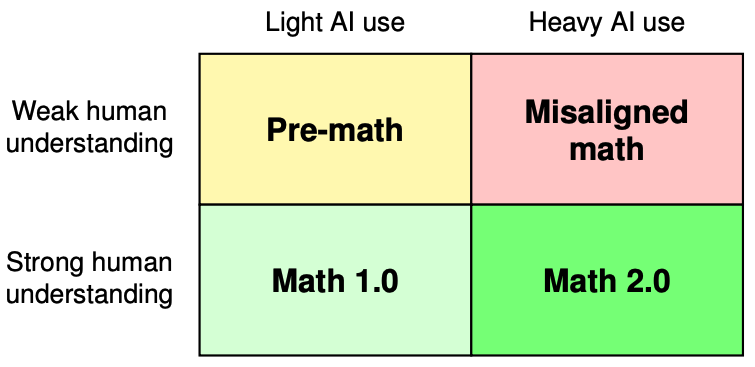
\includegraphics[width=6.8cm]{images/tao_math20.png}};
    % portrait, on a white disc with a soft shadow
    \node[circle, fill=white, inner sep=0pt, minimum size=2.02cm,
          drop shadow={shadow xshift=0.6pt, shadow yshift=-0.8pt, opacity=0.25}] at (11.3,-1.03) {};
    \node at (11.3,-1.03) {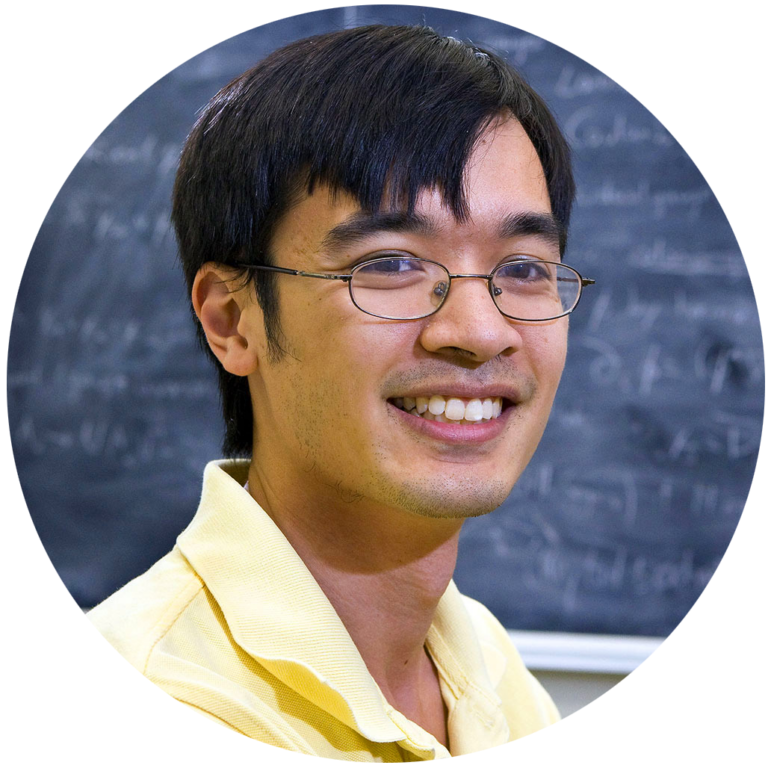
\includegraphics[width=1.92cm]{images/terry_tao.png}};
    % quote
    \node[anchor=north, text width=5.6cm, align=flush left, inner sep=0pt,
          font=\rmfamily\itshape\footnotesize] (q) at (11.35,-2.35)
      {{\color{black!50}\upshape[}{\color{black!55}Rather than blindly using AI to generate misaligned mathematics,}{\color{black!50}\upshape]}
       the more sustainable \textup{``Math 2.0''} use of AI would be to strengthen all the ways in which
       human understanding interacts with mathematics.};
    \node[anchor=north east, inner sep=0pt, font=\rmfamily\fontsize{26}{26}\selectfont, text=PennRed!80]
      at ([xshift=-0.05cm, yshift=0.12cm]q.north west) {``};
    % attribution
    \node[anchor=north west, inner sep=0pt, font=\sffamily\scriptsize, text=black!60, text width=6.0cm, align=left]
      at ([yshift=-0.22cm]q.south west)
      {--- Terence Tao, \emph{Machine Assisted Proof},\\AIM Public Lecture, Caltech, 9 Oct 2026};
    % thesis
    \node[anchor=south, draw=PennBlue!55, fill=PennBlue!4, line width=0.6pt, rounded corners=2pt,
          text width=11.4cm, inner xsep=0.3cm, inner ysep=0.2cm, align=left, font=\sffamily\small]
      at (7.13,-6.45)
      {\emph{
          For mathematicians, theorists, and theoretically-inclined experimentalists alike, gracefully and ethically navigating the transition to Math 2.0 will require reckoning with societal-level issues as well as developing individual familiarity with the emergent paradigm of AI-assisted formalization.
      %   Gracefully navigating the transition to Math~2.0 requires
      %  reckoning with societal level issues as well as understanding emerging best practices to capitalize
      %  on AI-driven workflows while maintaining scientific integrity, foremost by the principled integration of autoformalization into the theorists toolbox.
       }};
  \end{tikzpicture}
  \slidesources{Quote and diagram: T.~Tao, \emph{Machine Assisted Proof}, AIM Public Lecture Series, Caltech, 9 Oct 2026 (caltech.edu/campus-life-events/calendar/aim-public-lecture-series-terence-tao-1)}
\end{frame}

% [0.5 min] Overview: one card per part, listing that part's sections. The
% lists are generated from the section tree (\tableofcontents, subsections
% hidden), so they follow any change to the structure in main.tex.
% Beamer numbers the parts 1--4, so Part I is part=2 and Part II is part=3.
{
\setbeamertemplate{section in toc}{%
  \leavevmode\hbox to 0.9em{\color{PennRed}\rule[0.18ex]{0.42em}{0.42em}\hfil}%
  \inserttocsection\par}
\setbeamercolor{section in toc}{fg=black!80}
\newcommand{\overviewcard}[3]{% #1 label, #2 part name, #3 part number in the toc
  \begin{tikzpicture}[x=1cm, y=1cm, baseline={(0,0)}]
    \def\w{6.6}\def\h{4.4}\def\hb{1.25}
    \useasboundingbox (0,0) rectangle (\w,-\h);
    % card
    \fill[white, rounded corners=3pt,
          drop shadow={shadow xshift=0.6pt, shadow yshift=-0.8pt, opacity=0.25}] (0,0) rectangle (\w,-\h);
    % header band
    \begin{scope}
      \clip[rounded corners=3pt] (0,0) rectangle (\w,-\h);
      \fill[PennBlue] (0,0) rectangle (\w,-\hb);
      \fill[PennRed] (0,-\hb) rectangle (\w,{-\hb-0.06});
    \end{scope}
    \draw[black!15, line width=0.4pt, rounded corners=3pt] (0,0) rectangle (\w,-\h);
    \node[anchor=south west, inner sep=0pt, font=\sffamily\scriptsize\bfseries, text=white!70!PennBlue]
      at (0.45,-0.52) {\MakeUppercase{#1}};
    \node[anchor=north west, inner sep=0pt, font=\sffamily\Large, text=white]
      at (0.45,-0.6) {#2};
    % sections of this part
    \node[anchor=north west, inner sep=0pt, text width={\w cm - 0.9cm}, font=\sffamily\normalsize]
      at (0.45,{-\hb-0.05}) {\tableofcontents[part=#3, hideallsubsections]};
  \end{tikzpicture}%
}
\begin{frame}{The rest of this talk}
  \vspace*{0.87cm}
  \centering
  \overviewcard{Part I}{\partnameone}{2}\hspace{0.7cm}%
  \overviewcard{Part II}{\partnametwo}{3}
\end{frame}
}

              %  1.5 min

\part{\partnameone}                            % 15 min
\sectionslide{Part I}{\partnameone}
% Part I > Rampant AI use: the fact, and the problems it creates for checking
\section{Rampant AI use}

% [1.5 min] The fact of rampant AI use, and what it does to checking. Left:
% monthly share of arXiv math preprints that (blue) acknowledge AI use (Epoch),
% (orange) read as AI-written without disclosing AI writing (Martin; series
% starts Aug 2025), (purple) acknowledge AI for formalization (Epoch).
% Right: Kyle's four points, each with its numbers.
% Kyle's original bullets:
%   - Rampant AI use has led to exponentially increasing submissions to journals
%     and preprint servers, with an increasing number disclosing AI use
%   - However, many do not disclose. An increasing fraction are even thought to
%     be generated in whole by AI.
%   - OpenAI set the standard of accompanying results with formal certificates,
%     but relatively few are doing this, in particular in machine learning.
%   - (Other significant statistics regarding published work using AI)
% Data: research/03-publishing-crisis.md, "AI use, disclosure and formalization".
% Colours: tlBlue / tlOrange / tlPurple pass the dataviz palette validator.
\begin{frame}{The Poison Fountain}
  \centering
  \begin{tikzpicture}[x=1cm, y=1cm,
      claimnum/.style={circle, fill=PennRed, text=white, inner sep=0pt, minimum size=0.42cm,
                       font=\sffamily\scriptsize\bfseries},
      claim/.style={anchor=north west, text width=4.95cm, align=flush left, inner sep=0pt,
                    font=\sffamily\scriptsize, text=black!75}]
    \useasboundingbox (-0.4,0.15) rectangle (14.21,-6.35);
    % ---- chart -------------------------------------------------------------
    \node[anchor=north west, inner sep=0pt, font=\sffamily\scriptsize\bfseries, text=black!70]
      at (0.0,0.1) {Share of arXiv math preprints, by month};
    \begin{axis}[at={(1.0,-0.75)}, anchor=north west, scale only axis, width=6.55cm, height=4.75cm,
        xmin=-0.5, xmax=21.5, ymin=0, ymax=52, clip=false,
        xtick={0,6,12,18,21}, xticklabels={Jan '25, Jul '25, Jan '26, Jul '26, Oct},
        ytick={0,10,20,30,40,50}, yticklabel={\pgfmathprintnumber[assume math mode=true]{\tick}\%},
        tick label style={font=\sffamily\tiny, text=black!60},
        axis line style={draw=black!30}, tick style={draw=black!30},
        ymajorgrids, grid style={draw=black!8},
        axis x line*=bottom, axis y line*=left,
        legend style={at={(0.02,0.98)}, anchor=north west, draw=none, fill=white, fill opacity=0.9,
                      text opacity=1, font=\sffamily\tiny, row sep=-1pt, inner sep=1pt},
        legend cell align=left,
        every axis plot/.append style={line width=1.1pt, line join=round, mark size=0.75pt}]
      % disclosed AI use, any purpose (Epoch AI, recomputed from the 9 Nov 2026 CSV)
      \addplot[color=tlBlue, mark=*] coordinates {
        (0,0.35) (1,0.49) (2,0.23) (3,0.77) (4,0.80) (5,0.92) (6,0.86) (7,1.12) (8,1.74) (9,1.50) (10,1.36)
        (11,1.91) (12,1.93) (13,2.39) (14,3.68) (15,3.89) (16,6.64) (17,8.43) (18,15.42) (19,26.33) (20,38.55) (21,48.05)};
      \addlegendentry{Acknowledge AI use}
      % apparent AI writing with no disclosure of AI writing (Martin, 3 Nov 2026)
      \addplot[color=tlOrange, mark=*] coordinates {
        (7,4.9) (8,4.2) (9,5.0) (10,6.3) (11,5.5) (12,7.4) (13,7.4) (14,9.7) (15,12.2) (16,14.4)
        (17,16.2) (18,19.1) (19,21.1) (20,20.6) (21,17.5)};
      \addlegendentry{Read as AI-written, not disclosed}
      % AI acknowledged for formalization (Epoch AI)
      \addplot[color=tlPurple, mark=*] coordinates {
        (0,0) (1,0) (2,0) (3,0.03) (4,0) (5,0) (6,0) (7,0.03) (8,0.03) (9,0.02) (10,0.05)
        (11,0.05) (12,0.06) (13,0.17) (14,0.14) (15,0.39) (16,0.16) (17,0.55) (18,0.68) (19,1.31) (20,1.81) (21,1.88)};
      \addlegendentry{AI used for formalization}
      % end values, in text ink beside each line
      \node[anchor=west, font=\sffamily\tiny\bfseries, text=black!75] at (axis cs:21.4,48.05) {48\%};
      \node[anchor=west, font=\sffamily\tiny\bfseries, text=black!75] at (axis cs:21.4,17.5) {17.5\%};
      \node[anchor=west, font=\sffamily\tiny\bfseries, text=black!75] at (axis cs:21.4,1.88) {1.9\%};
    \end{axis}
    % ---- claims ------------------------------------------------------------
    \foreach \n/\y in {1/-0.05, 2/-1.65, 3/-3.25, 4/-4.85} \node[claimnum] at (8.95,\y-0.17) {\n};
    \node[claim] at (9.35,-0.05)
      {\textbf{\color{black}Use is exploding.} Disclosed AI use went from 0.4\% to 48\% of math
       preprints in 21 months, doubling about every three months. Math submissions are up
       75\% on a year earlier (Sep 2026).};
    \node[claim] at (9.35,-1.65)
      {\textbf{\color{black}Much of it is undisclosed.} About 1 in 6 math preprints read as AI-written
       without saying so. At ICLR 2026, 9\% of submissions were mostly AI-written.};
    \node[claim] at (9.35,-3.25)
      {\textbf{\color{black}Few certify.} OpenAI shipped Lean proofs with 42\% of its 719 manuscripts.
       Across arXiv math, 1.9\% acknowledge AI for formalization; in stat.ML, 0.4\% even mention Lean.};
    \node[claim] at (9.35,-4.85)
      {\textbf{\color{black}Review is overwhelmed.} 21\% of ICLR 2026 reviews were fully AI-generated.
       arXiv capped submissions (1 Oct); six probability journals paused (19~Oct\,--\,8~Nov).};
  \end{tikzpicture}
  \slidesources{Epoch AI (CC BY 4.0, 9 Nov 2026) \textbullet{} K.~Martin (3 Nov 2026) \textbullet{} our arXiv count \textbullet{} Pangram, ICLR 2026 (self-reported) \textbullet{} AcadMathSci, Oct 2026}
\end{frame}
              %  1.5 min  (the fact of rampant AI use)
% Part I > Community response: how the field reacted, and the problems each
% response exposes. Leads into section 12 (what formalization fixes).
% Facts and sources: research/03 (publishing), 05 (applied voices), 06
% (AcadMathSci report review). Corpus statistics: eda.py on data/dataset.csv.
\section{Community response}

% [1.5 min] The field agrees AI works; it disagrees about consequences.
% Statistics recomputed 2026-11-10 from data/dataset.csv with eda.py's filters
% (152 posts in the analysis set; 141 address capability). LLM-scored,
% self-selected corpus: illustration, not a survey.
% 49% = 75 of 152 with rubric 'overall' < 0 (10 at 0, 67 positive).
\begin{frame}{Proofs and Prompts: A Sentiment Analysis}
  \centering
  \begin{tikzpicture}[x=1cm, y=1cm]
    \useasboundingbox (0,0) rectangle (14.3,-6.3);
    \node[collagecard, anchor=north west] at (0,0)
      {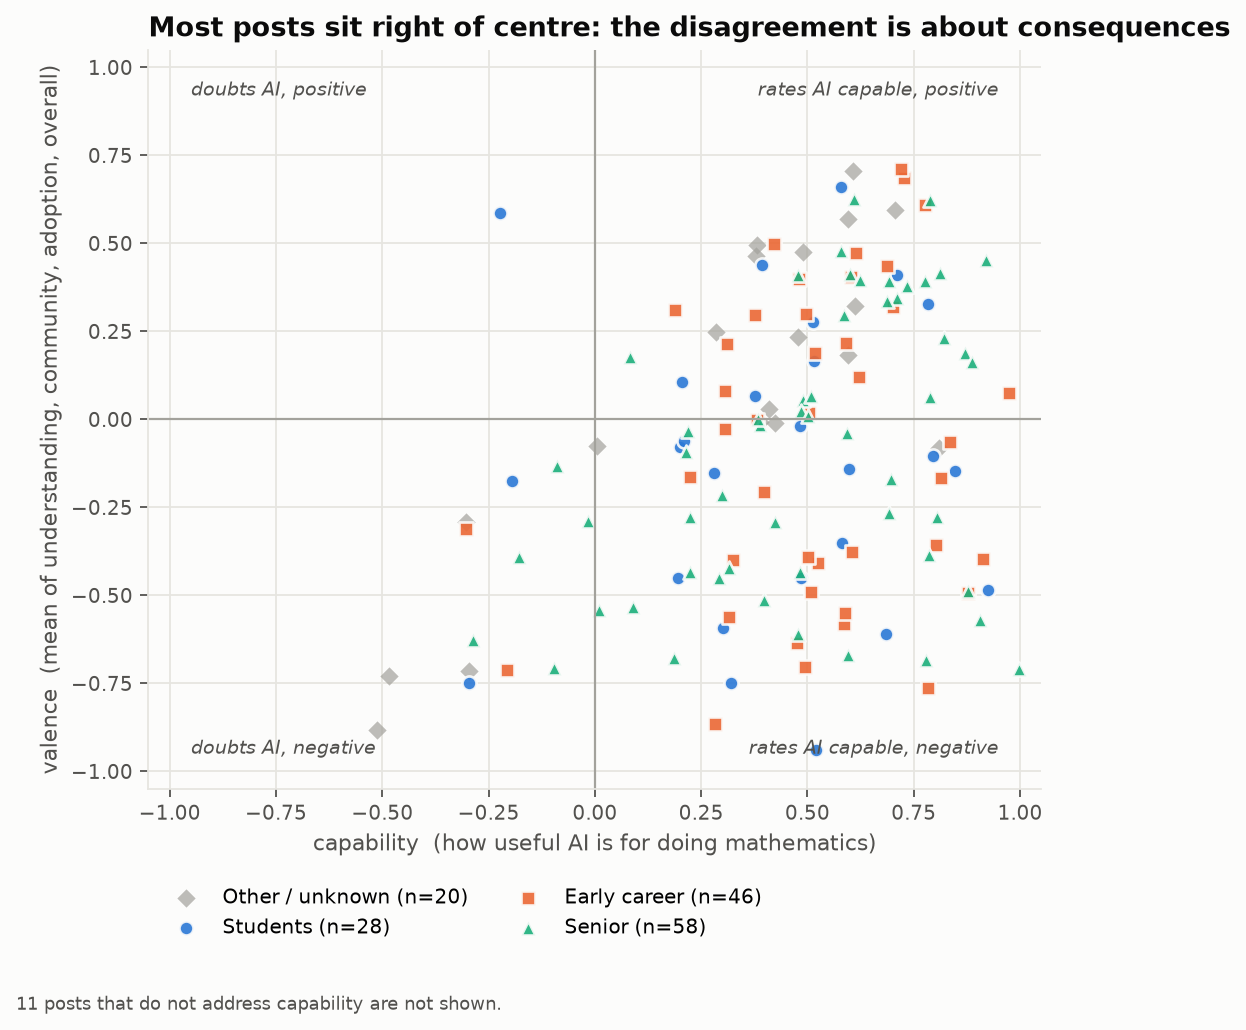
\includegraphics[height=6.1cm]{../figures/04_capability_vs_valence.png}};
    \node[anchor=north west, text width=6.2cm, align=flush left, inner sep=0pt,
          font=\sffamily\small] at (8.1,-0.35) {%
      {\color{black!55}\scriptsize 152 essays on \emph{proofsandprompts.com}, each scored by an LLM}\par\bigskip
      {\fontsize{22}{24}\selectfont\bfseries\color{tlBlue}89\%}\par
      rate AI as capable of doing mathematics\par\bigskip
      {\fontsize{22}{24}\selectfont\bfseries\color{tlOrange}49\%}\par
      view AI as a negative force overall\par\bigskip
      \textbf{The field agrees that it works.\\ It disagrees about the consequences.}};
  \end{tikzpicture}
  \slidesources{Proofs \& Prompts corpus (proofsandprompts.com), scored with Claude; analysis set of 152 posts, 141 addressing capability. Self-selected essays: an illustration, not a survey}
\end{frame}

% [1 min] The three clusters and the words that distinguish them. The method
% is kept off the slide (removed 2026-11-10); it is here for questions.
% Method (cluster.py, reviewed 2026-11-10): an LLM embeds each post in an
% interpretable semantic space (rubric.py: seven scored dimensions). Clustering
% uses two coordinates of that embedding, capability and valence (mean of
% understanding, community, adoption, overall), standardised, with k-means (k=3, 141 posts; silhouette 0.43, bootstrap ARI median 0.91).
% Cluster names come from a rule on the centres (name_cluster: capability >= 0.4
% -> "capable", else "doubted"; valence > 0.15 positive, < -0.15 negative). The
% "doubted" centre sits at capability +0.04, i.e. neutral rather than doubting.
% Word clouds are computed afterwards from the raw text: per-cluster log-odds of a term appearing in a post
% (z >= 2, >= 5 posts), with a hand-curated list of generic words removed.
\begin{frame}{Proofs and Prompts: What Each Cluster Writes About}
  \centering
  \begin{tikzpicture}[x=1cm, y=1cm]
    \useasboundingbox (0,0) rectangle (14.3,-5.95);
    % clusters in the score plane (figure is 0.872 wide per unit height: ~5.1 cm here);
    % cluster names, sizes and centres are labelled inside the figure
    \node[collagecard, anchor=north west] at (0,0)
      {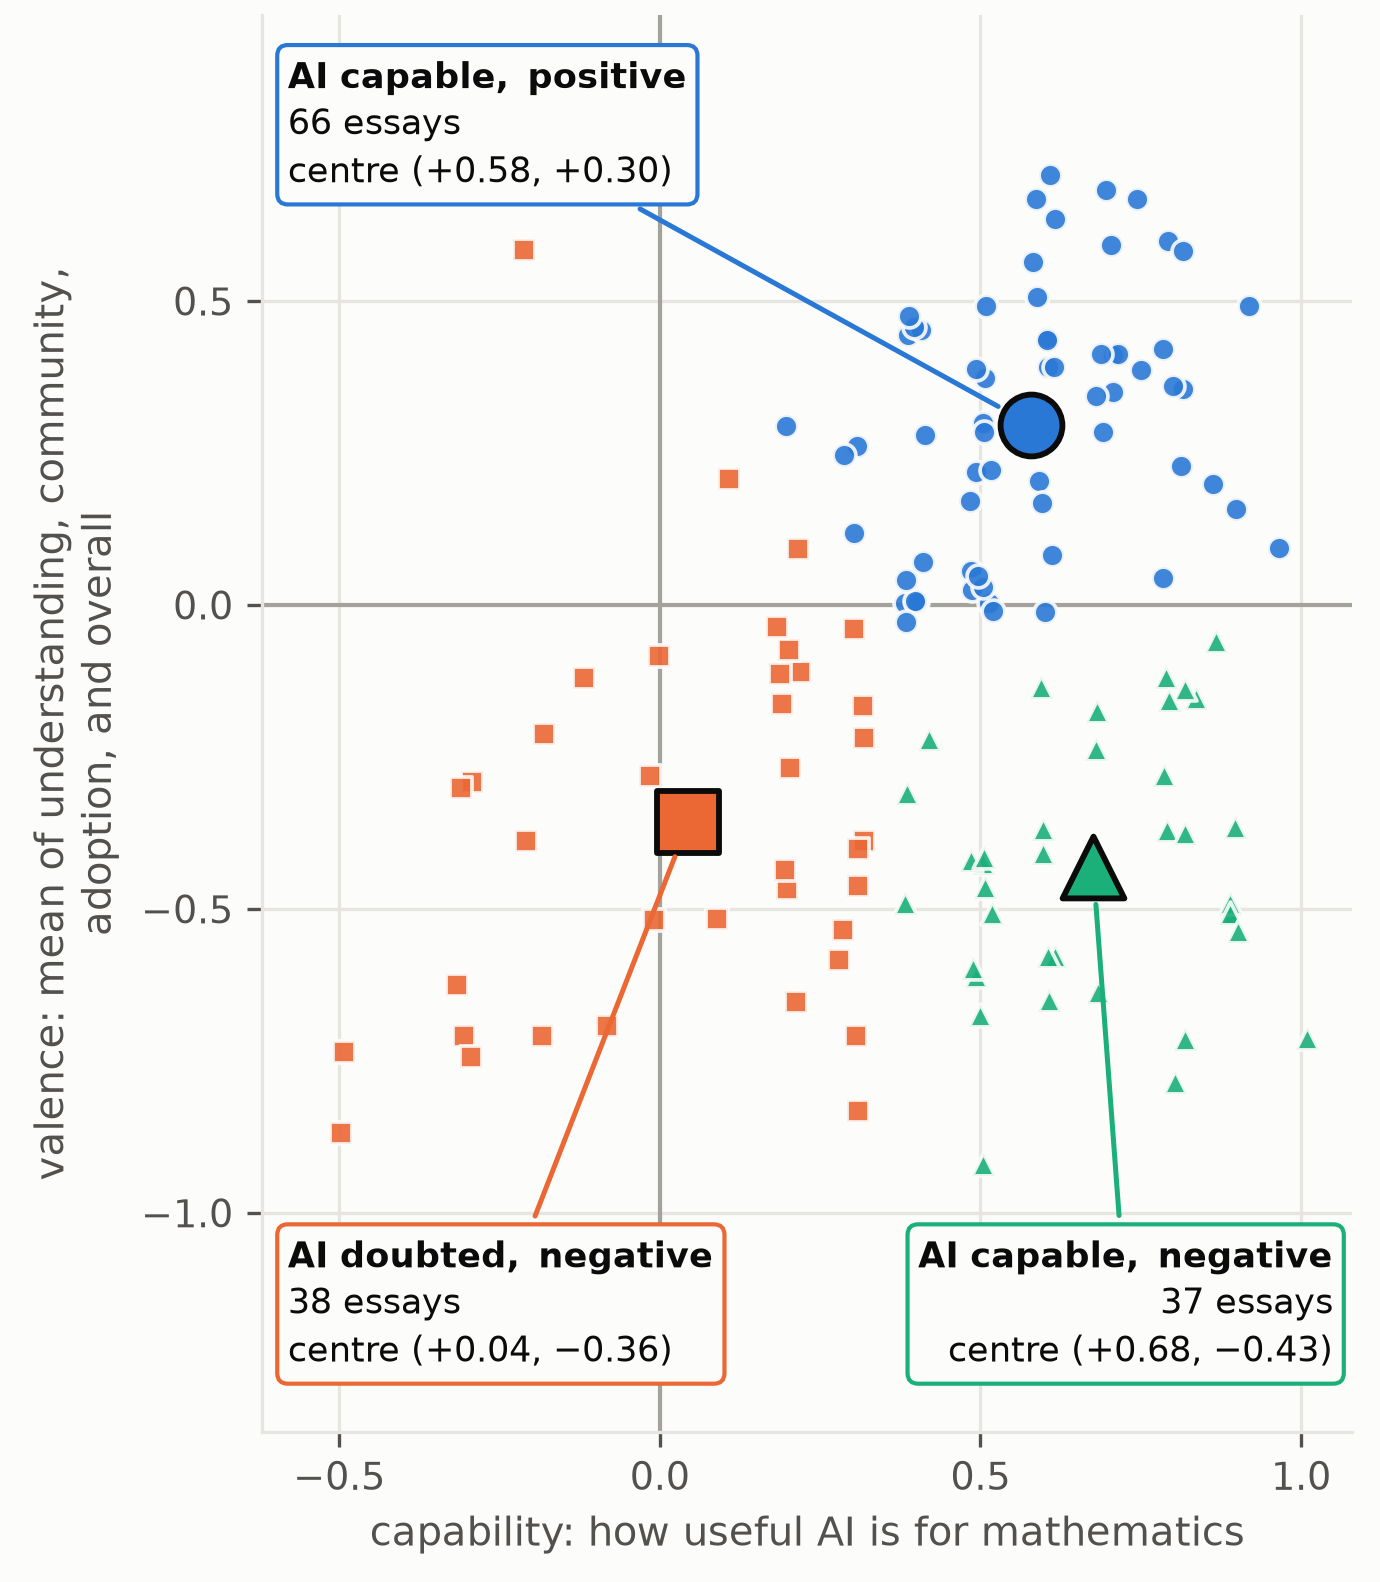
\includegraphics[height=5.85cm]{../figures/08_clusters.png}};
    % word clouds, one per cluster, stacked top to bottom in the same colours (2:3 figure)
    \node[collagecard, anchor=north east] at (14.3,0)
      {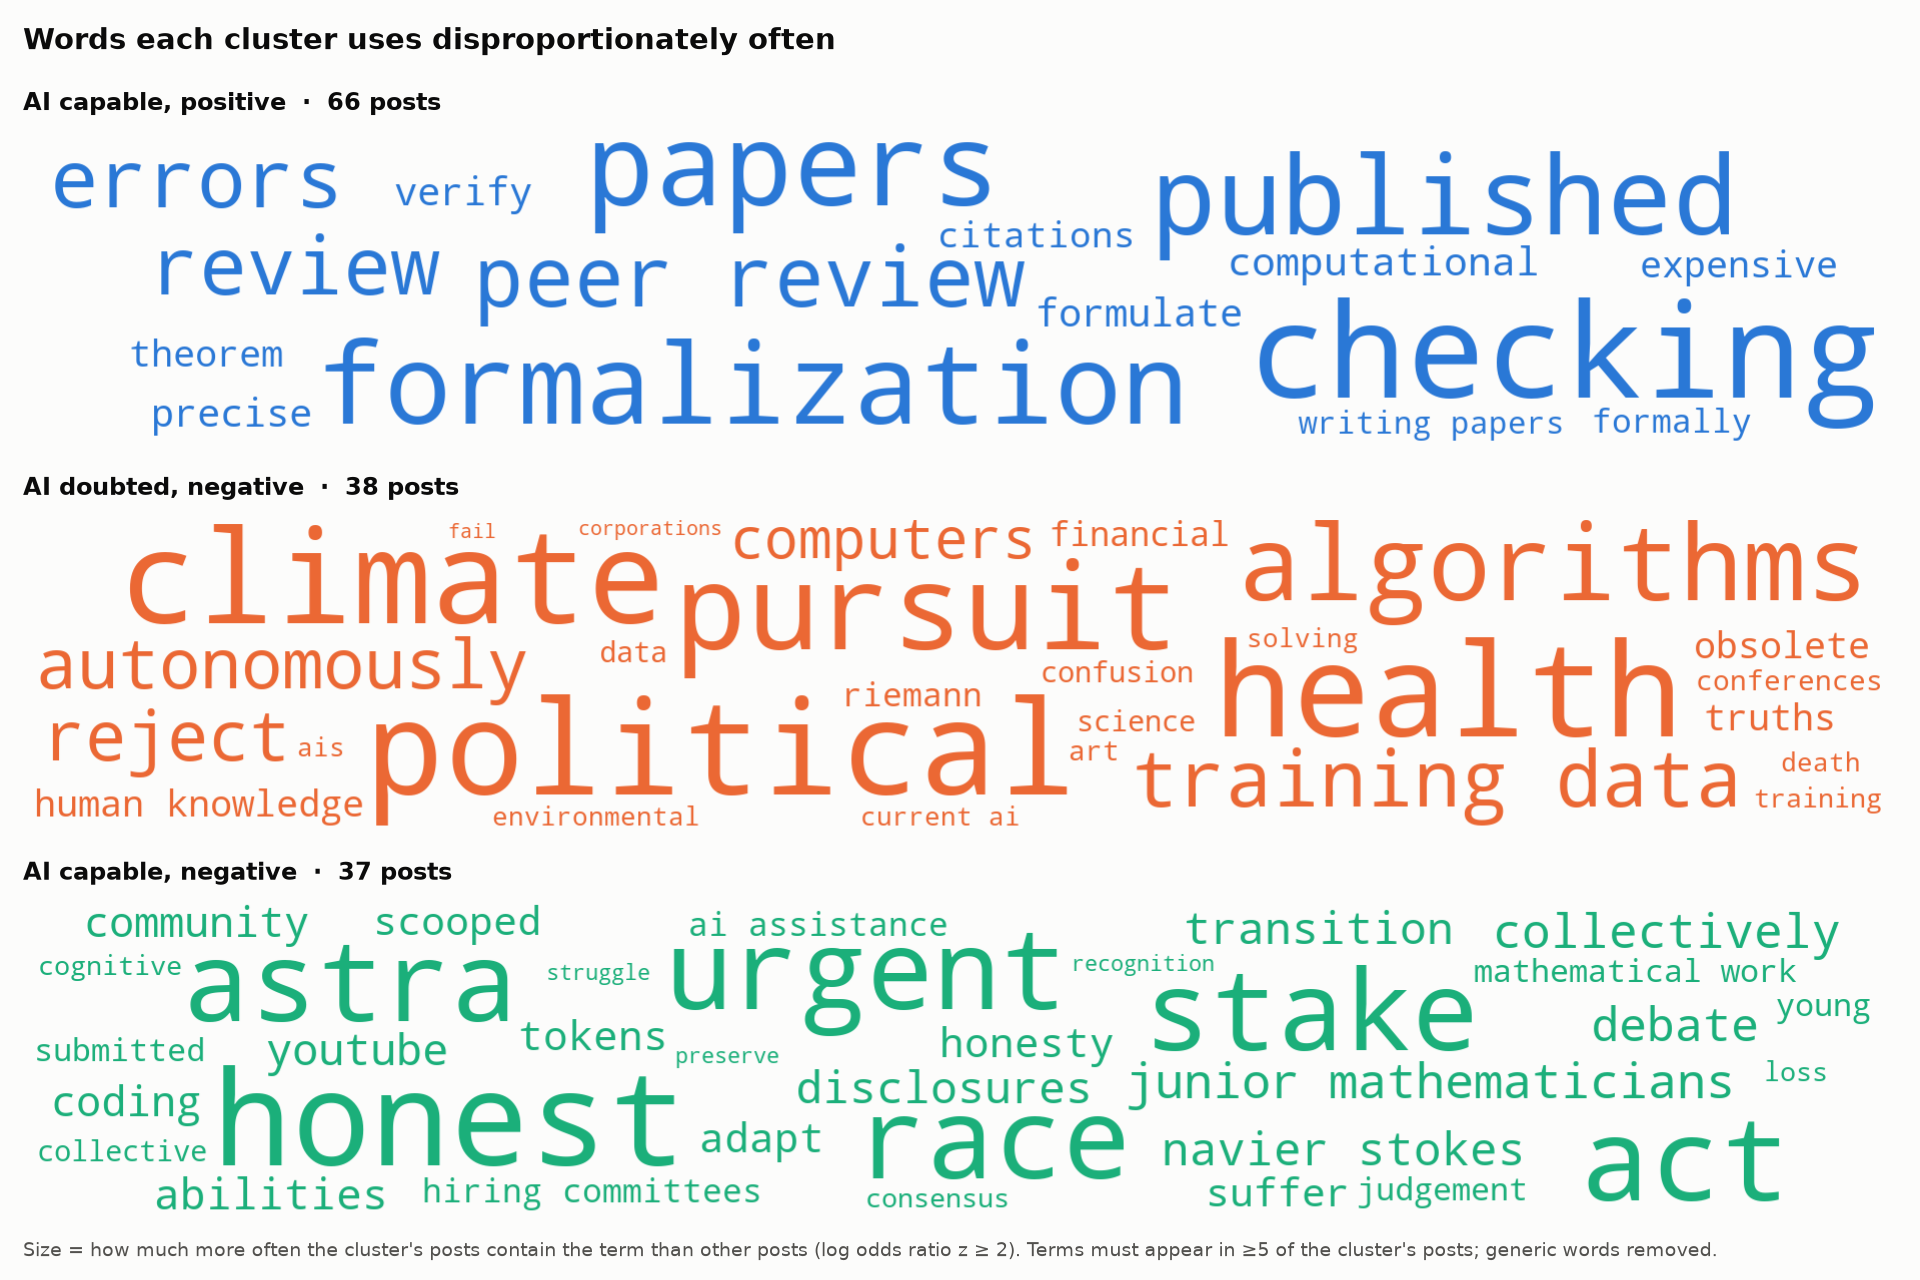
\includegraphics[height=5.85cm]{../figures/09_wordclouds.png}};
  \end{tikzpicture}
  \slidesources{Proofs \& Prompts corpus; scores from Claude (rubric.py); clustering and word statistics from cluster.py. Self-selected essays: an illustration, not a survey}
\end{frame}

% [2 min] Who did what, and who is told. Each row: the problem, the case that
% exposed it, the institutional response, and how far that response reaches.
\begin{frame}{Credit, disclosure and confidentiality}
  \footnotesize\sffamily
  \renewcommand{\arraystretch}{1.35}
  \begin{tabularx}{\linewidth}{@{}p{2.3cm}YYp{1.5cm}@{}}
    \toprule
    \tabhead{Problem} & \tabhead{Case} & \tabhead{Response} & \tabhead{Status}\\
    \midrule
    \rowhead{Credit} & AI reuses known ideas without attribution: 8 of Aletheia's 13 meaningful Erd\H{o}s results were already in the literature. Kolda: ``Human--AI scrapple''
      & Leiden Declaration (Jun 2026, endorsed by the IMU): human responsibility, attribution & \stpartial\\
    \rowhead{Priority} & Navier--Stokes priority dispute (C\'ordoba \& Mart\'inez-Zoroa; Buckmaster \& Alp\"oge)
      & AGMAI release guidelines (29 Sep): review before announcement, release prompts. Labs withheld prompts & \stopen\\
    \rowhead{Disclosure} & 1 in 6 math preprints read as AI-written without saying so. At ICML 2026, 22.5\% of reviewers used an LLM under a ban
      & Disclosure statements (arXiv, Springer, Leiden); SIAM AI policy v2.0 & \stpartial\\
    \rowhead{Confidentiality} & Referees uploading manuscripts to AI tools
      & LMS: misconduct. SIAM v2.0: ``non-delegation of scholarly judgement'' & \stpartial\\
    \bottomrule
  \end{tabularx}\par\medskip
  {\color{black!60}\scriptsize The rules already bind individuals; none of them can be checked from the paper alone.}
  \slidesources{Reisinger et al., AcadMathSci, Oct 2026 (A.3, C.1, C.4, C.5) \textbullet{} Kolda, Silicon Reckoner, Feb 2026 \textbullet{} Martin, Nov 2026 \textbullet{} Kim et al., arXiv 2609.19420}
\end{frame}

% [1.5 min] Volume against fixed refereeing capacity.
\begin{frame}{Review capacity}
  \footnotesize\sffamily
  \renewcommand{\arraystretch}{1.35}
  \begin{tabularx}{\linewidth}{@{}p{2.3cm}YYp{1.5cm}@{}}
    \toprule
    \tabhead{Problem} & \tabhead{Case} & \tabhead{Response} & \tabhead{Status}\\
    \midrule
    \rowhead{Volume} & arXiv math: 7,428 submissions in Sep 2026, against 4,252 a year earlier (+75\%). A few prolific authors drive much of it
      & arXiv: two new submissions per submitter per month (1 Oct). STOC 2027: at most five per author & \stdone\\
    \rowhead{Referees} & Six probability journals paused new submissions (19 Oct\,--\,8 Nov). Editors report they cannot find a referee
      & Pauses; proposals for paid, AI-assisted refereeing (Maltsev) & \stopen\\
    \rowhead{AI reviewing} & ICLR 2026: 21\% of reviews fully AI-generated
      & ICLR plans automated screening of reviews and submissions & \stpartial\\
    \rowhead{Bypassed review} & Results announced on X and GitHub before any review (Navier--Stokes; 719 manuscripts in a day)
      & Leiden and AGMAI: announce through peer review. Palomar registry of Lean-verified results (18 Aug); a proposed journal requiring Lean proofs (Guo, 17 Oct) & \stpartial\\
    \bottomrule
  \end{tabularx}\par\medskip
  {\color{black!60}\scriptsize Restricting and disclosing are in place; verifying is the structural response, and it is still a prototype.}
  \slidesources{AcadMathSci, Oct 2026 (\S1.2) \textbullet{} Nee, Zhong \& Ni, arXiv 2609.04872 \textbullet{} Fortnow, Sep 2026 \textbullet{} Pangram, ICLR 2026 (self-reported) \textbullet{} Tao, blog, 18 Aug and 17 Oct 2026}
\end{frame}

% [1.5 min] Who learns, who can afford it, and what gets studied.
\begin{frame}{Training, access and narrowing}
  \footnotesize\sffamily
  \renewcommand{\arraystretch}{1.35}
  \begin{tabularx}{\linewidth}{@{}p{2.3cm}YYp{1.5cm}@{}}
    \toprule
    \tabhead{Problem} & \tabhead{Case} & \tabhead{Response} & \tabhead{Status}\\
    \midrule
    \rowhead{Training} & Students given unrestricted GPT-4 scored 17\% lower once access was removed; a tutor with guardrails largely avoided the harm (Bastani et al.)
      & Vivas and in-person exams; AI-permitted work graded on formulation and validation & \stpartial\\
    \rowhead{Access} & Only 11\% of researchers have institutional funding for their main AI tool (Springer Nature, 10,480 researchers). Navier--Stokes cost an estimated \pounds4.9M
      & Token costs eligible on grants (proposed); SAIR Open Math OS: free open models for academics & \stpartial\\
    \rowhead{Narrowing} & AI adoption shrinks topic range by 4.6\% and engagement by 22\% (Hao et al., 41M papers). Agendas drift toward ``problems easily amenable to current AI''
      & Reward understanding and long-term contribution over volume (AcadMathSci) & \stopen\\
    \bottomrule
  \end{tabularx}
  \slidesources{Reisinger et al., AcadMathSci, Oct 2026 (\S1.6, \S3.2, \S3.3, \S4.3, B.1) \textbullet{} Bastani et al., PNAS \textbullet{} Hao et al., arXiv 2412.07727}
\end{frame}
         %  6.5 min  (the response exposes the problems)
% Part I > What formalization fixes: the problems the community response
% exposed, what a machine-checked certificate (used correctly) does about each,
% where it stops (Navier--Stokes), and the open problems handed to Part II.
% Facts and sources: research/01 (s5, Navier--Stokes and the OpenAI audit),
% 02 (Palomar, Comparator, Prove2Me), 03 (s5, what formalization can and
% can't do).
\section{What formalization fixes}

% [2 min] Introduces AI-assisted formalization as a concept: the pipeline
% (human statement and blueprint -> AI formalizes and proves -> kernel checks
% -> registered certificate), then what it addresses from the community-response
% section and what it leaves open. Replaces the earlier problem/certificate
% table (same content, Kyle asked for a non-table slide).
\begin{frame}{AI-assisted formalization}
  \centering
  \begin{tikzpicture}[x=1cm, y=1cm, font=\sffamily\footnotesize]
    \useasboundingbox (0,0.1) rectangle (14.3,-5.9);
    % ---- definition --------------------------------------------------------
    \node[anchor=north west, text width=14.2cm, align=flush left, inner sep=0pt, font=\sffamily\small]
      at (0,0.05)
      {AI translates mathematics into a proof assistant such as Lean and fills in the proofs.
       A small trusted kernel checks every step. Humans write, or review, what is being proved.};
    % ---- pipeline ----------------------------------------------------------
    \node[stage=PennBlue, minimum width=2.9cm, minimum height=1.05cm] (p1) at (1.65,-1.5)
      {Statement \& blueprint\\[-1pt]{\scriptsize\color{black!60}human}};
    \node[stage=tlPurple, minimum width=2.9cm, minimum height=1.05cm] (p2) at (5.35,-1.5)
      {Formalize \& prove\\[-1pt]{\scriptsize\color{black!60}AI agents}};
    \node[stage=PennGreen, minimum width=2.9cm, minimum height=1.05cm] (p3) at (9.05,-1.5)
      {Kernel check\\[-1pt]{\scriptsize\color{black!60}Lean}};
    \node[stage=PennGold, minimum width=2.9cm, minimum height=1.05cm] (p4) at (12.75,-1.5)
      {Certificate\\[-1pt]{\scriptsize\color{black!60}registry, e.g.\ Palomar}};
    \foreach \u/\v in {p1/p2, p2/p3, p3/p4} \draw[flow] (\u) -- (\v);
    \draw[flow=PennBlue, dashed] (p3.south) .. controls +(0,-0.55) and +(0,-0.55) .. (p1.south);
    \node[note, fill=white, inner sep=1pt] at (5.35,-2.48) {a human checks that the formal statement matches the paper};
    % ---- what it addresses / what stays open --------------------------------
    \node[anchor=north west, inner sep=0pt, font=\sffamily\small\bfseries, text=PennGreen] at (0,-2.95)
      {What it addresses};
    \node[anchor=north west, inner sep=0pt, font=\sffamily\small\bfseries, text=PennRed] at (7.35,-2.95)
      {What stays open};
    \node[anchor=north west, text width=6.85cm, align=flush left, inner sep=0pt, font=\sffamily\scriptsize] at (0,-3.4) {%
      \begin{itemize}\setlength{\itemsep}{1pt}
        \item \textbf{Review capacity.} Referees review a page of statements, not 60 pages of proof.
        \item \textbf{Undisclosed AI.} The check does not depend on who, or what, wrote the proof.
        \item \textbf{Bypassed review.} Verify and register a result before announcing it.
        \item \textbf{Credit.} Registries record what produced each result.
      \end{itemize}};
    \node[anchor=north west, text width=6.85cm, align=flush left, inner sep=0pt, font=\sffamily\scriptsize] at (7.35,-3.4) {%
      \begin{itemize}\setlength{\itemsep}{1pt}
        \item \textbf{Statement fidelity.} Compiling is not saying the same thing (Navier--Stokes).
        \item \textbf{Understanding.} Millions of machine-written lines explain nothing.
        \item \textbf{Significance and ideas.} Neither is a formal property.
        \item \textbf{Access and coverage.} Frontier compute; thin libraries in PDE and applied probability.
      \end{itemize}};
  \end{tikzpicture}
  \slidesources{Tao, \emph{Palomar}, blog, 18 Aug 2026 \textbullet{} Bastounis, Circelli \& Hansen, arXiv 2610.08144 \textbullet{} research notes 01--03}
\end{frame}

% [1.5 min] Navier--Stokes revisited: the certificate compiled, and the code
% still says something other than the paper. They do NOT claim the paper is
% wrong; the argument was about credit, not correctness.
\begin{frame}{The paper and the code disagree}
  \small\sffamily
  \begin{columns}[T]
    \begin{column}{0.54\textwidth}
      \textbf{Navier--Stokes} (Bastounis, Circelli \& Hansen, Oct 2026)
      \begin{itemize}\footnotesize
        \item The paper's estimate (8.19) needs $m{+}4$ derivatives; the matching Lean theorem assumes $m{+}5$, and the pattern repeats.
        \item The paper's pressure bound depends on one quantity; the Lean bound depends on two, and is proved by a different route.
        \item They do not claim the paper is wrong.
      \end{itemize}
      \medskip
      \textbf{OpenAI's 719 manuscripts} (community audit of 245 formalized families)
      \begin{itemize}\footnotesize
        \item About 210 consistent at the level of statements; no theorem shown false.
        \item 21 headline results marked ``(Lean)'' were not formalized; 5 formalized only a supporting lemma.
      \end{itemize}
    \end{column}
    \begin{column}{0.42\textwidth}
      \vspace{0.4cm}
      \begin{tikzpicture}
        \node[draw=PennRed!45, fill=PennRed!3, line width=0.6pt, rounded corners=2pt,
              text width=5.3cm, inner sep=0.3cm, align=left, font=\rmfamily\itshape\small] (q)
          {Lean acceptance (compilation) of translation does not imply semantic preservation.};
        \node[anchor=north west, font=\sffamily\scriptsize, text=black!60, inner sep=0pt]
          at ([yshift=-0.15cm]q.south west) {--- Bastounis, Circelli \& Hansen, arXiv 2610.08144};
      \end{tikzpicture}
      \vspace{0.5cm}

      {\footnotesize A certificate proves \emph{a} theorem. Whether it is \emph{the} theorem is a human question.}
    \end{column}
  \end{columns}
  \slidesources{Bastounis, Circelli \& Hansen, arXiv 2610.08144 \textbullet{} borism/openai-math-slop, issue \#2 \textbullet{} research note 01, \S5}
\end{frame}

% [2 min] The three layers: posed here, answered in Part II.
\begin{frame}{Three layers of checking}
  \centering
  \begin{tikzpicture}[x=1cm, y=1cm]
    \useasboundingbox (0,0.1) rectangle (14.2,-6.0);
    \node[layer=PennGreen, anchor=north west] (k) at (3.6,0)
      {\textbf{Does Lean accept the proof?} Cheap and mechanical. Watch for \texttt{sorry}, extra axioms and kernel bugs.\hfill{\stdone}};
    \node[lbl=PennGreen] at (3.35,-0.72) {1. Kernel};
    \node[layer=PennGold, anchor=north west] (s) at (3.6,-1.8)
      {\textbf{Does the formal statement say what the paper claims?} Scarce: ``will never be solved purely in software'' (Kontorovich). Navier--Stokes drifted here.\hfill{\stopen}};
    \node[lbl=PennGold!85!black] at (3.35,-2.52) {2. Statement};
    \node[layer=PennRed, anchor=north west] (u) at (3.6,-3.6)
      {\textbf{Does anyone understand the proof, and does it match the written one?} Scarce. Machine proofs run to millions of lines.\hfill{\stopen}};
    \node[lbl=PennRed] at (3.35,-4.32) {3. Understanding};
    \node[anchor=north, font=\sffamily\small, text width=12cm, align=center] at (7.8,-5.4)
      {Layer 1 is solved. Layers 2 and 3 are the open problems for AI-assisted formalization: Part II.};
  \end{tikzpicture}
  \slidesources{Research note 01, \S0 \textbullet{} Kontorovich, via AcadMathSci, Oct 2026 (\S2.2) \textbullet{} Bastounis, Circelli \& Hansen, arXiv 2610.08144}
\end{frame}
       %  5.5 min  (what formalization fixes; what stays open)

\part{\partnametwo}                            % 20 min
\sectionslide{Part II}{\partnametwo}
% Part II > In our field (hook)
\section{In our field}

\begin{frame}{Formalization reaches learning theory}
  \stub{1.5}{Hook: people in our field are already doing this}
\end{frame}

\begin{frame}{No verifier, no flywheel}
  \stub{1}{Why pure math moved first and where our field sits}
\end{frame}

                  %  2.5 min
% Part II > How it is being done (tools + practice)
\section{How it is being done}

\begin{frame}{The tools}
  \stub{1}{One layered map: copilot, project, engine, library}
\end{frame}

\begin{frame}{A spectrum of human direction}
  \stub{1}{From fully automatic to human-led; one real case per point}
\end{frame}

\begin{frame}{Fully automatic}
  \stub{1}{Case}
\end{frame}

\begin{frame}{Agents on a human roadmap}
  \stub{1}{Case}
\end{frame}

\begin{frame}{AI filling a human blueprint}
  \stub{1}{Case}
\end{frame}

\begin{frame}{Human-led, AI-assisted}
  \stub{1}{Case}
\end{frame}

             %  6   min
% Part II > What we can do > The three layers
\section{What we can do}
\subsection{The three layers}

\begin{frame}{Running example}
  \stub{1}{A lemma from the lab's own work, carried through the layers}
\end{frame}

\begin{frame}{Kernel: reading a Lean file}
  \stub{2}{What compiles, and what can hide inside it}
\end{frame}

\begin{frame}{Statement: humans own the statements}
  \stub{2.5}{Statement review; the part software cannot do}
\end{frame}

\begin{frame}{Understanding: blueprints and hand-picked lemmas}
  \stub{2}{Human-facing narrative over a machine-built proof}
\end{frame}

              %  7.5 min  (What we can do > The three layers)
% Part II > What we can do > In the lab
\subsection{In the lab}

\begin{frame}{What to hand to AI}
  \stub{1}{The convex hull; what stays human}
\end{frame}

\begin{frame}{Experiments and applied work}
  \stub{1}{Code, tests and validation as the certificate}
\end{frame}

\begin{frame}{Budget}
  \stub{1}{Compute costs for a student or a lab}
\end{frame}

\begin{frame}{Checklist}
  \stub{1}{Each item tied to a layer}
\end{frame}

                 %  4   min  (What we can do > In the lab)

\part{Closing}                                 %  3 min
\sectionslide{}{Closing}
% Closing: individual responsibility; full circle with the opener; call to action
\section{Closing}

\begin{frame}{Where this leaves us}
  \stub{0.5}{Recap: (a) what is coming (Society), (b) how to take part (The Lab)}
\end{frame}

\begin{frame}{Proof abundance, insight scarcity}
  \stub{1}{Full circle with the opener and Tao: certificates make proofs abundant; insight is what stays scarce, and it lives in individuals}
\end{frame}

\begin{frame}{Stay the author}
  \stub{1}{Individual responsibility: keep control of what is generated, keep your own insights, do not cede your perspective to AI}
\end{frame}

\begin{frame}{A call to action}
  \stub{0.5}{A few personal commitments for each person in the room}
\end{frame}

\begin{frame}{Discussion}
  \stub{--}{Prompts to open the 15 minutes}
\end{frame}
                    %  3   min

\appendix
% Backup
\section{Backup}

\begin{frame}{Corpus and scoring method}
  \stub{--}{Details behind the opinion map}
\end{frame}

\begin{frame}{Backup slides}
  \stub{--}{Material for questions}
\end{frame}

\begin{frame}{References}
  \stub{--}{Sources}
\end{frame}



\end{document}
